% Companion chapter to MTP_FINAL_REPORT.tex.  This source is intentionally
% explanatory: it is a guided, source-audited tour rather than pasted code.
\section{How to Read and Reconstruct This Implementation}
\label{sec:walkthrough}
This section is written for a reader who knows elementary graph theory and C++ but has not read Ibarra's paper or this repository.  It explains, in dependency order, \emph{which question each module answers}, \emph{which invariant it maintains}, \emph{what the actual frozen C++ does}, and \emph{why the work bound follows}.  The report first develops the static objects (a PEO, maximal cliques, a clique tree), then the four chordality-preserving operations, then the data structures needed to speed up the operations.  It finishes with executable verification and known limitations.

\paragraph{Source and reproducibility contract.}
All filenames below are paths relative to the GitHub repository linked on the cover.  Code and statements refer to frozen implementation SHA \texttt{2bf723c2b3b57a6b532058f21742b8125292852a}; documentation commits on \texttt{main} do not change the core.  A function name denotes the \emph{actual C++ implementation}; a reference to Ibarra's numbered section denotes the published method.  When the code uses a representation improvement or a subsequent published building block, this distinction is identified explicitly.  The report is meant to be read alongside, but is not a replacement for, the source listings.  The exact repository tree contains more comments, test inputs, error messages, and internal consistency checks than would be practical to reproduce verbatim in a thesis.

\subsection{A five-minute conceptual map}
The mathematical object we maintain is a \emph{clique tree}: every node represents one \emph{maximal clique} of the current graph, and every ordinary tree edge is labelled by the size of the intersection of its endpoint cliques.  A vertex appearing in several maximal cliques must appear in every clique on the tree path connecting them.  This \emph{running-intersection} property is what makes local edge updates possible.

The software has three layers:
\begin{enumerate}[leftmargin=*]
\item \textbf{Static graph layer.} Store the current undirected graph, find a perfect elimination ordering by Maximum Cardinality Search (MCS), verify chordality, enumerate maximal cliques, and build a weighted clique tree.
\item \textbf{Dynamic chordal layer.} For an edge \(uv\), decide whether its deletion is safe; for a nonedge \(uv\), decide whether its insertion is safe.  If safe, perform an Ibarra clique-tree transformation without recomputing all maximal cliques.  A1 uses an ordinary tree adjacency list; A2 adds a specialized dynamic forest and a full clique-intersection table.
\item \textbf{Optional accelerations and a different graph class.} A1+ and A2+ accelerate deletion queries with a member/overflow index.  A separate degree-sequence data structure maintains split-graph recognition under arbitrary \emph{valid} edge notifications.
\end{enumerate}
This layering matters: the simple chordality criteria should be understood \emph{before} the more elaborate A2 data structures.  The faster tree cannot repair an incorrect graph-theoretic criterion.

\subsection{Notation used consistently throughout}
Let \(G=(V,E)\) be a simple undirected graph, \(|V|=n\), \(|E|=m\); let \(\mathcal K=\{K_1,\ldots,K_c\}\) be all maximal cliques.  A clique \(K\) is maximal when it is not properly contained in a larger clique; \emph{maximal} is not synonymous with \emph{maximum}.  Let \(T\) be a tree on those cliques.  Write
\[
T_v=\{x:v\in K_x\},\quad S_{xy}=K_x\cap K_y,\quad
w(x,y)=|S_{xy}|\ (xy\in E(T)),\quad W[x,y]=|K_x\cap K_y|.
\]
Here \(w\) labels \emph{tree edges}, whereas \(W\) is the cardinality of the intersection of \emph{any} two cliques, adjacent or not.  A path bottleneck is
\(\lambda(x,y)=\min_{e\in P_T(x,y)}w(e)\).  In general \(\lambda(x,y)\ge W[x,y]\); equality need not hold.  This distinction is essential to the insertion query.

\subsection{An example we use repeatedly}
The repository file \path{data/example_7_vertices.txt} contains \(n=7,m=10\), with edges
\[
\{01,13,02,23,24,25,45,36,03,12\}.
\]
Its three maximal cliques are, ignoring their possibly different output IDs,
\[
K_A=\{0,1,2,3\},\qquad K_B=\{2,4,5\},\qquad K_C=\{3,6\}.
\]
They form the clique tree \(K_B- K_A- K_C\), with separator labels \(1\) and \(1\): \(K_A\cap K_B=\{2\}\), \(K_A\cap K_C=\{3\}\).  The three clique nodes containing vertex \(2\) are actually \(K_A,K_B\), and the clique nodes containing vertex \(3\) are \(K_A,K_C\); both are connected as the running-intersection property requires.  Vertex \(6\) appears only in \(K_C\).

\begin{center}
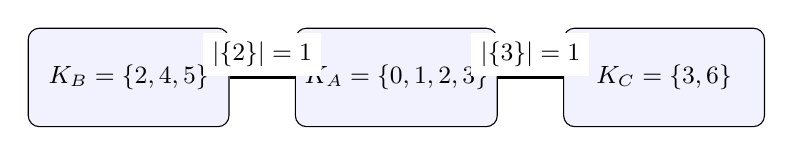
\begin{tikzpicture}[every node/.style={font=\small},x=3.4cm,y=1cm]
\node[draw,rounded corners,fill=blue!5,minimum width=2.55cm,minimum height=1.25cm] (B) at (0,0) {$K_B=\{2,4,5\}$};
\node[draw,rounded corners,fill=blue!5,minimum width=2.55cm,minimum height=1.25cm] (A) at (1,0) {$K_A=\{0,1,2,3\}$};
\node[draw,rounded corners,fill=blue!5,minimum width=2.55cm,minimum height=1.25cm] (C) at (2,0) {$K_C=\{3,6\}$};
\draw[thick] (B)-- node[above,fill=white] {$|\{2\}|=1$} (A);
\draw[thick] (A)-- node[above,fill=white] {$|\{3\}|=1$} (C);
\end{tikzpicture}
\end{center}
This figure is \emph{the actual graph's clique tree}, not an arbitrary illustrative drawing.  The node numbering used by the program can differ because MCS tie-breaking determines enumeration order; the \emph{sets and intersection weights} are the invariant information.

\section{Detailed C++ Graph and Input Representation}
\label{sec:graph-impl}
\subsection{Why two adjacency representations are maintained}
The \path{Graph} class (\path{include/mtp/graph.hpp}, \path{src/graph.cpp}) stores \texttt{adjacency\_} as \texttt{vector<vector<int>>} and \texttt{neighbor\_sets\_} as \texttt{vector<set<int>>}.  The vector is used to scan every neighbour in \(O(\deg(v))\), crucial for MCS, PEO checking, and clique construction.  The balanced set answers \texttt{has\_edge(u,v)} in worst-case \(O(\log(n+1))\), avoiding an expected-time hash-table claim.  Both representations are updated whenever an edge changes; their agreement is an invariant.

\paragraph{Insertion.} \texttt{add\_edge} validates both IDs, rejects a self-loop, inserts endpoints in their respective balanced sets, appends the neighbour IDs to both vectors, and increments the edge count.  Duplicate calls do not increase the count.  Set work is \(O(\log n)\) worst-case; the vector append is amortized \(O(1)\) but individually can take \(O(n)\) because of reallocation, still within A1's total \(O(n)\) worst-case operation allowance.

\paragraph{Deletion.} \texttt{remove\_edge} erases both set entries and uses erase/remove to remove the neighbour IDs from both adjacency vectors.  Vector scanning costs \(O(\deg u+\deg v)\subseteq O(n)\), so one graph deletion is worst-case \(O(n)\).  A reader should not infer \(O(\log n)\) for the \emph{whole} graph-edge deletion from the presence of the two balanced sets alone.

\subsection{The bulk constructor and its linear-time rationale}
When measuring A1 \emph{initialization}, the graph must be loaded in the claimed time, not supplied by an uncounted \(m\)-step incremental process.  The implementation \texttt{Graph::from\_edges(n,edges)} traverses each input edge \(\{u,v\}\) once and records the directed half-edges in buckets indexed by the \emph{neighbor} ID.  It then processes buckets in increasing index order.  This makes each source vertex's adjacency vector sorted without a comparison sort:
\begin{lstlisting}[language=C++,caption={Conceptual bulk-loader loop; see src/graph.cpp.}]
for (auto [u,v] : edges) {
    by_neighbor[v].push_back(u);
    by_neighbor[u].push_back(v);
}
for (int neighbor = 0; neighbor < n; ++neighbor)
    for (int source : by_neighbor[neighbor])
        adjacency[source].push_back(neighbor);
for (int v = 0; v < n; ++v)
    neighbor_sets[v] = std::set<int>(adjacency[v].begin(),
                                    adjacency[v].end());
\end{lstlisting}
The real code additionally validates endpoints, rejects loops and duplicate adjacency entries, and maintains the edge count.  Bucket handling visits \(2m\) half-edges and \(n\) buckets.  Construction of each \texttt{std::set} from an already sorted range has the standard linear-time range-construction guarantee, so the total is \(O(n+m)\) under the C++17 standard library cost model.  The A1 CLI uses this bulk constructor.  The A2 CLI currently reads with individual \texttt{Graph::add\_edge} calls; its input-loading cost must therefore be \emph{separately} considered when claiming an end-to-end A2 preprocessing bound.

\paragraph{Input contract.} A graph file begins with \texttt{n m}, followed by exactly \texttt{m} undirected pairs \texttt{u v}, with IDs \(0,\ldots,n-1\).  The CLI rejects a missing file, invalid header, malformed list, and trailing tokens.  Nonchordal initial graphs are rejected by the dynamic chordal constructors; permissible \emph{updates} preserve chordality by a query-before-mutation rule.

\section{Maximum Cardinality Search and PEO Verification}
\label{sec:mcs-detail}
\subsection{Why a PEO is needed}
An ordering \(v_1,\ldots,v_n\) is a \emph{perfect elimination ordering} when, for every \(i\), all neighbours of \(v_i\) occurring later in the order are mutually adjacent.  The chordal-graph theorem states that a finite simple graph is chordal if and only if it has a PEO.  This supplies a linear-time recognition route and the structure from which all maximal cliques can be recovered.  An arbitrary ordering is not sufficient: a four-cycle with no diagonal has no PEO, so clique-tree processing must not silently continue on it.

\subsection{Precisely what the MCS implementation does}
In \texttt{maximum\_cardinality\_search}, each unnumbered vertex \(v\) has an integer \texttt{weight[v]}, equal to the number of already chosen neighbours.  At every step choose an unnumbered vertex of maximum weight, place it at the rightmost still-vacant position in \texttt{ordering}, and increase the weight of each unnumbered neighbour.  The chosen vertices therefore appear in reverse selection order in the returned PEO candidate.

The code uses \texttt{vector<list<int>> buckets(n)}, a list for every possible integer weight, and \texttt{locations[v]}, a linked-list iterator identifying exactly where the vertex currently sits.  The invariant is:
\[
  v\text{ is unnumbered}\implies v\in\texttt{buckets[weight[v]]}
  \text{ exactly once}.
\]
Moving a vertex from bucket \(k\) to bucket \(k+1\) is \(O(1)\) using the saved iterator.  A \texttt{max\_weight} pointer identifies the largest nonempty bucket and is lowered while necessary.  Initialization costs \(O(n)\), and each undirected edge causes at most a constant number of neighbour-weight updates; thus the whole algorithm costs \(O(n+m)\) time and space.  Its deterministic use of \texttt{push\_front} fixes a reproducible, but not uniquely mathematically required, tie-breaking order.

\begin{lstlisting}[caption={MCS logic, simplified from src/mcs.cpp.}]
for (position = n-1; position >= 0; --position) {
    while (max_weight > 0 && buckets[max_weight].empty())
        --max_weight;
    chosen = buckets[max_weight].front();
    erase chosen from its bucket;
    ordering[position] = chosen;
    numbered[chosen] = true;
    for (neighbor : adjacency[chosen]) if (!numbered[neighbor]) {
        remove neighbor by locations[neighbor];
        ++weight[neighbor];
        push neighbor into buckets[weight[neighbor]];
        locations[neighbor] = iterator to new list entry;
    }
}
\end{lstlisting}
\subsection{Why MCS output still needs verification}
MCS returns an elimination candidate for \emph{any} graph.  For chordal input, the relevant MCS theorem guarantees a PEO.  On a nonchordal graph, returning an integer order is not proof of chordality.  The code explicitly calls \texttt{is\_perfect\_elimination\_ordering} before maximal-clique or dynamic initialization.  This is both a correctness gate and a useful design boundary.

\subsection{The linear-time PEO verifier, line by line}
Let \texttt{position[u]} be the location of vertex \(u\) in the proposed order.  Define its \emph{earliest later neighbour} \(p(u)\) as the later neighbour with minimum position, or \(-1\) if none.  A PEO has the equivalent property
\[
 N^+(u)\setminus\{p(u)\}\ \subseteq\ N(p(u))
\qquad\text{for every }u\text{ with }p(u)\neq-1.
\]
The verifier first checks that \texttt{ordering} is exactly a permutation of the vertices.  Then one adjacency pass computes \texttt{parent[u]=p(u)}.  It groups all \(u\) with the same parent into \texttt{children[p]}.  For each parent \(p\), it marks \(N(p)\) \emph{once} in a temporary array; then it checks the later neighbours of every \(u\in\texttt{children[p]}\).  An unmarked later neighbour other than \(p\) violates the criterion, and the function returns false.

The grouping is important: marking \(N(p(u))\) afresh for every \(u\) could repeat expensive adjacency scans.  In the actual implementation, each parent neighbourhood is marked at most once and each child's neighbourhood is inspected once; the total work is \(O(n+m)\).  Neither an adjacency matrix nor randomised hashing is needed.  If \(n=0\), the empty order is valid; the code's boundary cases are explicitly tested.

\section{Maximal Cliques and the Blair--Peyton Clique Tree}
\label{sec:bp-detail}
\subsection{Why candidate cliques appear in a PEO}
For each vertex \(u\) in a PEO define
\[
 C(u)=\{u\}\cup N^+(u),\qquad N^+(u)=\{v:uv\in E,\ \operatorname{pos}(v)>\operatorname{pos}(u)\}.
\]
By definition of PEO, \(C(u)\) is a clique.  Every maximal clique is one of these candidate cliques: take its earliest vertex \(u\), observe that every other member is a later neighbour, and use maximality.  But not every \(C(u)\) is maximal; duplicates or proper subsets must be filtered.

The verification/reference extractor \texttt{extract\_maximal\_cliques} computes the later-neighbour list and earliest later parent \(p(u)\).  It uses the known parent--subsumption condition: when \(u\) has parent \(p\) and
\[
 |N^+(u)|-1=|N^+(p)|,
\]
then the candidate belonging to \(p\) is subsumed by \(C(u)\) and should not be separately emitted.  Its \texttt{maximal} flags suppress such candidates before producing the final vector of cliques.  This module is useful for independent checking of the production constructor; it is \emph{not} the quadratic clique-intersection-graph algorithm.

\subsection{Why we did not build an explicit all-pairs clique graph in production}
A straightforward route to a clique tree is to enumerate all maximal cliques, build a weighted graph whose nodes are cliques and whose edge weights are their intersection sizes, and find a maximum-weight spanning tree.  This is a sound reference/oracle construction, but up to \(c\le n\) maximal cliques give \(\Theta(c^2)\) pairs.  A long star graph is an instructive example: its maximal cliques are \(\{0,i\}\), one for each leaf, so the clique intersection graph contains quadratically many positive edges even though the input has only \(n-1\) edges.  Using it as production preprocessing would forfeit the desired \(O(n+m)\) bound.

We therefore preserve the explicit weighted clique graph and Kruskal constructor only as \emph{reference implementations} in \path{src/clique_graph.cpp} and \path{src/clique_tree.cpp}.  The production constructor is \texttt{build\_clique\_tree\_blair\_peyton} in \path{src/clique_tree_blair_peyton.cpp}.

\subsection{Step-by-step Blair--Peyton implementation}
Blair--Peyton's expanded-MCS construction is linear on chordal input.  The code receives the MCS-derived PEO and verifies it first.  It constructs \texttt{position[v]} and \texttt{clique\_of\_vertex[v]}, then walks the PEO \emph{backwards}.

For the current \(u\), let \texttt{current\_card} be the number of later neighbours already numbered and let \texttt{previous\_card} be the corresponding count at the preceding reverse iteration.  The implementation starts a new maximal-clique node precisely when \texttt{current\_card <= previous\_card}; the initial value of \texttt{previous\_card} is zero.  The new node initially receives the later neighbours of \(u\).  The current vertex \(u\) is then inserted into whichever clique node is active.

When a new clique has a nonempty later-neighbour set, the code chooses the \emph{minimum-position later neighbour} \(p\).  The existing clique containing that vertex, obtained from \texttt{clique\_of\_vertex[p]}, is the new node's parent in the clique tree.  The tree edge is labelled \texttt{current\_card}, exactly the common-separator size from the expanded-MCS construction.  When there are no later neighbours, we have entered a disconnected component; the code joins the new component's clique tree to the existing forest by a \emph{dummy tree edge of weight zero}.  This ensures the dynamic algorithms can represent disconnected input by one connected clique tree without treating the dummy as an original graph edge.

\begin{lstlisting}[caption={Conceptual expanded MCS, matching the frozen constructor.}]
for (index = n-1; index >= 0; --index) {
    u = peo[index];
    higher = {v in N(u) : position[v] > index};
    current_card = higher.size();
    if (current_card <= previous_card) {
        s = create clique node containing higher;
        if (current_card > 0)
            link(s, clique_of_vertex[earliest(higher)],
                 current_card);
        else if (an older component exists)
            link_dummy(s, first_component_clique, 0);
    }
    s = most recently created clique node;
    clique_of_vertex[u] = s;
    append u to clique K_s;
    previous_card = current_card;
}
\end{lstlisting}
\paragraph{Why the total work stays linear.} Every original vertex is processed once; every adjacency list is visited at most a constant number of times; the total number of vertices appearing in maximal cliques is at most \(n+m\) (Lemma~\ref{lem:incidence}); each clique-tree edge is added once.  The resulting \(O(n+m)\) time bound does not depend on a dense pairwise matrix.

\subsection{What makes a clique-tree result correct}
The test suite independently checks four things after construction and after each permitted dynamic update: (1) the set of clique nodes equals the actual maximal cliques obtained afresh from the graph, after canonical sorting; (2) the number of tree edges is \(c-1\) for \(c>0\); (3) each stored edge weight matches the true intersection cardinality of its endpoints; and (4) for every graph vertex \(v\), the clique nodes containing \(v\) are connected when we restrict a BFS to those nodes.  These are stronger checks than merely asking that a function return success or that the resulting graph remain chordal.

\section{The Two Published Chordality Criteria}
\label{sec:criteria-detail}
\subsection{Deletion criterion: exactly one maximal clique}
Let \(uv\in E(G)\).  Ibarra's Theorem~4 states
\[
G-uv\text{ chordal}\quad\Longleftrightarrow\quad
\#\{K\in\mathcal K:\{u,v\}\subseteq K\}=1.
\]
The intuitive obstruction is an induced four-cycle that appears after removing the chord \(uv\).  If two distinct maximal cliques contain \(u,v\), each can contribute a different vertex opposite the removed chord.  Conversely, the uniqueness condition prevents such a witness.  The reader should notice that this is not equivalent to saying \(uv\) belongs to any clique---every existing edge does.  The \emph{number} of maximal cliques is decisive.

\paragraph{Small example.} In a complete triangle \(\{a,b,c\}\) the edge \(ab\) lies in exactly one maximal clique.  Removing it yields the two-edge path \(a-c-b\), still chordal.  In the graph formed from two triangles \(\{u,v,a\}\) and \(\{u,v,b\}\) sharing the edge \(uv\), that edge lies in two maximal cliques; removing it creates the chordless cycle \(u-a-v-b-u\).  A direct edge-deletion query must reject the second case.

\subsection{Insertion criterion: nearest cliques and two different numbers}
Let \(uv\notin E(G)\).  Because each \(T_u\) and \(T_v\) is connected, there is a well-defined shortest path between the two disjoint clique subtrees.  Let \(x\in T_u\), \(y\in T_v\) be the closest endpoints, and let \(P=P_T(x,y)\).  Ibarra's criterion is
\[
G+uv\text{ chordal}\quad\Longleftrightarrow\quad
\min_{e\in P}w(e)=|K_x\cap K_y|,
\]
with the adjacent-endpoints case satisfying equality automatically.  Operationally, choose one minimum-weight edge on \(P\); equality permits replacing that edge by \(xy\) before constructing the new clique.  If the path bottleneck is larger than the true endpoint intersection, the proposed edge induces an obstruction and must be rejected.

\paragraph{Why the two quantities are not interchangeable.} Consider three maximal cliques along a path:
\[
K_1=\{a,b,x\},\qquad K_2=\{a,b,c\},\qquad K_3=\{b,c,y\}.
\]
Both adjacent separators have cardinality two, yet \(K_1\cap K_3=\{b\}\) has cardinality one.  Thus \(\lambda(K_1,K_3)=2\ne W[1,3]=1\).  Inserting \(xy\) creates the induced four-cycle \(x-a-c-y-x\) (none of its diagonals is present), correctly rejected by Ibarra.  Computing only a minimum edge weight by an LCA/Kruskal reconstruction tree would produce the wrong decision.  The fast A2 representation must preserve the \emph{true} intersection information, not just the bottleneck.

\subsection{Why the closest pair can be found with a tree traversal}
\(T_u\) and \(T_v\) are connected subtrees of the same tree.  A multi-source BFS starting simultaneously at every node of \(T_u\) visits clique-tree nodes in increasing distance from that subtree.  The first node belonging to \(T_v\) therefore has minimum possible distance to \(T_u\).  Parent pointers recovered during BFS locate the corresponding node of \(T_u\) and the unique path.  This is the A1 implementation; the A2 implementation instead employs one witness in each subtree and \emph{binary search on the dynamic-tree path}.

\section{A1: Sparse Clique Membership, Operations and Correctness}
\label{sec:a1-full}
\subsection{The exact data structures in the preferred implementation}
The preferred class is \texttt{SparseIbarraChordalGraphA1} in \path{include/mtp/sparse_ibarra_a1.hpp} and \path{src/sparse_ibarra_a1.cpp}.  It stores the graph \texttt{graph\_}, a vector \texttt{nodes\_} of clique nodes, a vector \texttt{edges\_} of weighted clique-tree edges, \texttt{nodes\_of\_[v]} inverse lists, and free-ID lists for reuse.  A node has \texttt{active}, \texttt{members}, \texttt{inverse\_iterators}, and \texttt{incident}.  The member list contains only vertices actually belonging to the clique; there is no \(n\)-entry bitmap stored for each clique.  Every \texttt{inverse\_iterators[i]} points to the matching entry in \texttt{nodes\_of\_[members[i]]}.

Tree edges store endpoint clique IDs, the separator cardinality, and two linked-list iterators identifying their positions in the incident-edge lists of both endpoints.  Cutting an existing edge therefore removes the two list entries in constant time.  The implementation never relies on a hash lookup to locate the stored edge's list nodes.  This detail is important when claiming \(O(n)\) worst-case clique-tree maintenance.

\paragraph{Why explicit inverse iterators matter.} Suppose a clique \(x\) loses the member \(v\).  Searching \(T_v\) for \(x\) would cost \(O(|T_v|)\).  Repeating that search for every removed member could lead to quadratic update work.  Instead, \texttt{replace\_members(x,new\_members)} erases each prior inverse record using its saved iterator, replaces the member vector, and appends one inverse record per new member, storing the new iterators.  The cost is linear in the number of members removed and inserted, at most \(O(n)\) for each of the constant number of cliques rewritten by one A1 update.  The running \texttt{membership\_count\_} is updated for testing and memory accounting.

\paragraph{Recycled IDs.} \texttt{retire\_node} first verifies that a clique has no remaining incident tree edges, removes every inverse membership, clears its member vector and marks it inactive, then pushes the ID onto \texttt{free\_nodes\_}.  \texttt{allocate\_node} reuses a free ID or the next available fixed-capacity slot, installs its actual members, and increments the active count.  Keeping IDs bounded by \(n+2\) supports \(O(n)\)-sized scratch arrays; it also prevents dangling tree references, because a node cannot be retired before being detached.

\subsection{A1 Delete-Query: precisely what the code does}
\begin{enumerate}[leftmargin=*]
\item Validate \(u,v\); a self-pair is not an edge.  Return \textsf{no} if the current graph does not contain \(uv\).
\item Build an \(O(n)\)-length temporary byte vector indexed by clique-node ID, initially zero.
\item Mark every clique node listed in \texttt{nodes\_of\_[u]}; scan \texttt{nodes\_of\_[v]}.  The method \texttt{clique\_of\_edge} returns the unique common node ID if there is exactly one, otherwise \(-1\).
\item Answer \textsf{yes} precisely in the unique-clique case, as required by Ibarra's Theorem~4.
\end{enumerate}
The two inverse lists contain at most \(c\le n\) entries each; marking and scanning cost \(O(n)\).  The optional fast-index case delegates to the separately priced \texttt{FastCliqueIntersectionIndex} and is \emph{not} counted as the base A1 query data structure.

\subsection{A1 Delete: exact clique-tree transformation}
Assume \(uv\) is an existing edge and the query returns \textsf{yes}.  It belongs to one maximal clique \(K_x\), whose size is \(k\).  The deletion creates up to two candidate cliques
\[
K_{xu}=K_x\setminus\{v\},\qquad K_{xv}=K_x\setminus\{u\}.
\]
All other old maximal cliques remain maximal.  A candidate may nevertheless be \emph{subsumed} by an old neighbour clique, and the code must contract it if so.

The implementation first gathers members of both candidates by one scan through \texttt{nodes\_[x].members}.  It marks the inverse lists \(T_u\) and \(T_v\) into a two-bit temporary array.  For every neighbour clique \(y\) of \(x\) it determines which side should receive the old tree edge: \(N_u\) if \(y\) contains \(u\), \(N_v\) if it contains \(v\), or the remaining class.  Under the unique-clique deletion precondition a neighbour cannot contain both \(u\) and \(v\); otherwise there would be a second maximal clique containing the deleted edge.

A candidate \(K_{xu}\) is nonmaximal exactly when an appropriate \(N_u\)-neighbour has intersection weight \(k-1\) with \(K_x\).  Similarly, a \(k-1\) intersection in \(N_v\) identifies an absorbing clique for \(K_{xv}\).  The code therefore records \texttt{absorb\_u} and \texttt{absorb\_v} while classifying neighbours---there is no separate all-clique subset search.

Next, all old incident edges of \(x\) are detached; \(x\) is rewritten as \(K_{xu}\); a new node \(x_2\) represents \(K_{xv}\); the old neighbours are reattached to the proper side; and \(x-x_2\) is linked with separator size \(k-2\), the cardinality of \(K_x\setminus\{u,v\}\).  Finally each subsumed candidate is contracted into its recorded absorbing neighbour.  Only after these structural changes does the graph itself remove \(uv\).  The optional A1+ index, if enabled, is notified of changed cliques and rebalanced.

\paragraph{A concrete reversible deletion.} Suppose the current graph is the triangle \(\{u,v,a\}\).  Delete \(uv\): initially there is a single clique \(\{u,v,a\}\); afterwards \(\{u,a\}\) and \(\{v,a\}\) are the maximal cliques, connected by a tree edge of weight \(1\) for separator \(\{a\}\).  Reinsert \(uv\) and the two edge-cliques are replaced by the original triangle, with redundant endpoints contracted.  This tests both creation and absorption paths.

\paragraph{Complexity.} The query and two member scans cost \(O(n)\); marks and neighbour classification touch \(O(n)\) clique IDs/edges; link, cut and contraction use a total of \(O(n)\) constant-time adjacency-list modifications; and graph deletion costs at most \(O(n)\).  Thus \textsf{Delete} is \(O(n)\) worst case.  It does not require the dynamic Sleator--Tarjan forest.

\subsection{A1 Insert-Query: full BFS-to-criterion pipeline}
Assume \(uv\notin E\).  \texttt{closest\_pair(u,v)} creates a target marker for all nodes in \(T_v\) and enqueues all nodes of \(T_u\) as BFS sources.  Each initial source has its own parent pointer, pointing to itself.  At the first dequeued node in \(T_v\), it backtracks through parent and edge-ID arrays until it reaches one of the original sources.  The output is the closest pair \((x,y)\) and the ordered list of path-edge IDs.  A connected clique tree guarantees this search succeeds even when the original graph has multiple connected components joined by zero-weight dummy edges.

\texttt{overlap(x,y)} uses a temporary \(n\)-byte vertex marker, marks every vertex of \(K_x\), and scans \(K_y\); this yields \(I=|K_x\cap K_y|\) in \(O(n)\).  A separate pass over the path edges finds \(\lambda(x,y)\).  The query accepts exactly when \(\lambda(x,y)=I\).  No dense matrix is needed in A1, and the total is \(O(n)\) worst-case.

\subsection{A1 Insert: exchange, create, and absorb}
An accepted insertion can start with two endpoint cliques whose path in the old tree has many edges.  If the path has more than one edge, the program cuts an edge of minimum separator weight and links the endpoint cliques with the \emph{same} common-intersection weight, converting the tree into the adjacent-endpoint case described by Ibarra's Theorems~5--6.  This exchange is safe \emph{only because} the insertion query established equality with \(I\).

It then computes
\[
K_z=(K_x\cap K_y)\cup\{u,v\}
\]
using a one-pass vertex marker, removes the current \(xy\) tree edge, creates \(z\), and links \(x-z\) and \(z-y\) with weights \(I+1\).  Why \(I+1\)? Because \(K_x\cap K_z=I\cup\{u\}\), and analogously \(K_y\cap K_z=I\cup\{v\}\).

The endpoints may themselves cease to be maximal:
\[
K_x\subset K_z\iff |K_x|=I+1,\qquad
K_y\subset K_z\iff |K_y|=I+1.
\]
These are equality tests on clique size and intersection cardinality, not expensive subset comparisons.  The code contracts exactly those endpoint nodes whose equality condition holds.  At most two nodes can be subsumed; no unrelated maximal clique can become a proper subset of \(K_z\), by the separator structure in Ibarra's proof.

\paragraph{Worked insertion using the repository example.} Initially \(K_A=\{0,1,2,3\}\) and \(K_B=\{2,4,5\}\) are adjacent, with intersection \(I=\{2\}\).  Inserting \(04\) is legal.  It creates \(K_z=\{0,2,4\}\).  Since \(|K_A|=4>2\) and \(|K_B|=3>2\), neither original clique is absorbed; \(K_z\) is inserted between them with new tree-edge weights two.  Now deleting the recently inserted edge \(04\) is legal, because \(K_z\) is the unique clique containing it.  Deletion creates \(\{0,2\}\) and \(\{2,4\}\), but they are subsumed by \(K_A\) and \(K_B\), respectively, and the original clique tree is restored.

By contrast, in the restored original graph, consider inserting \(46\).  The closest cliques are \(K_B\) and \(K_C\), with path through \(K_A\).  The minimum tree-edge weight on that path is one, whereas \(K_B\cap K_C=\emptyset\), so \(1\ne0\) and the insertion must be rejected.  This explicitly demonstrates the bottleneck-versus-intersection comparison.

\paragraph{Complexity.} A second BFS, a path-minimum scan, marker construction, at most one new clique and at most two contractions require \(O(n)\) work.  Although the program can reroute \(\Theta(n)\) incident edges in a contraction, each linked-list link/cut is \(O(1)\) in A1.  This yields \(O(n)\) worst-case insertion.  The A2 version requires separate treatment because its forest links/cuts are \(O(\log n)\), not \(O(1)\).

\subsection{Why initial sparse incidence fits in \(O(n+m)\)}
The number of inverse-list records is exactly \(\sum_{K\in\mathcal K}|K|\).  Let \(v_K\) be the earliest PEO vertex of clique \(K\); the maximality and PEO properties imply \(K=\{v_K\}\cup N^+(v_K)\), and distinct maximal cliques cannot have the same earliest vertex.  Hence
\[
\sum_{K\in\mathcal K}|K|
\le\sum_{v\in V}(1+|N^+(v)|)=n+m.
\]
The program allocates \(O(n)\) node slots and inverse-list heads and one record per actual incidence, without constructing \(c\) length-\(n\) bitmaps.  This is the implementation-level repair of the original characteristic-vector initialization gap.  It changes the storage representation and some local primitive code, but not the Ibarra acceptance conditions or clique-tree transformations.  The optional fast-delete index deliberately reintroduces quadratic storage and must be charged separately.

\section{A2: Why a Faster Query Needs a Dynamic Forest and Matrix}
\label{sec:a2-full}
\subsection{The representation maintained in frozen A2}
The production A2 class is \texttt{SleatorTarjanChordalGraphA2} (\path{include/mtp/dynamic_ibarra_a2.hpp}, \path{src/dynamic_ibarra_a2.cpp}).  It owns four linked components:
\begin{enumerate}[leftmargin=*]
\item \texttt{DynamicChordalGraph data\_}: the old \emph{dense} clique representation and linked-list clique tree, kept because A2 needs \(O(1)\) vertex membership tests along a dynamically searched path.
\item \texttt{SleatorTarjanWorstCaseForest tree\_}: the same clique-tree topology represented using the globally biased Sleator--Tarjan worst-case dynamic forest.  The ordinary list tree and ST forest are synchronised via link/cut hooks.
\item \texttt{vertex\_witness\_[v]}: one active clique ID containing \(v\), sufficient to start the fast closest-pair search.
\item \texttt{W\_[x][y]}: explicit integer cardinalities of the intersections \(K_x\cap K_y\), for all active clique-node pairs.  This must be maintained after every successful update.
\end{enumerate}
A successful A2 update must preserve \emph{all four} invariants simultaneously.  If the clique tree is right but a witness points to a deleted clique, the next query can fail.  If the ST tree has correct edges but \(W\) is stale, it can make a wrong chordality decision.  If the matrix is correct but the ST path order or minimum is wrong, the binary search fails.  The implementation therefore includes explicit consistency checks and independent forest invariant tests.

\subsection{How frozen A2 initializes a nonempty graph}
Unlike the optimized A1 constructor, A2 does \emph{not} simply take Blair--Peyton's final cliques and fill \(W\) in a sparse way.  Its frozen source follows Ibarra Section~5.1's \emph{reverse PEO replay} option.  It begins with an empty graph on \(n\) vertices, where each vertex is initially a singleton maximal clique.  It links disconnected singleton clique trees by zero-weight dummy edges, initializes witnesses and the all-zero matrix \(W\) with singleton diagonals equal to one, attaches the ST link/cut hooks, and then inserts each original edge in reverse PEO order.  This insertion order is chosen because each intermediate subgraph is chordal, so all replayed operations satisfy the dynamic algorithm's precondition.  The result is the requested initial graph together with its fully updated clique tree, matrix and forest.

This construction is conceptually valuable but expensive.  It allocates \(n\) length-\(n\) characteristic vectors and an \((n+2)\times(n+2)\) integer matrix before replay.  Thus it uses \(\Omega(n^2)\) eager initialization even on \(m=0\).  The replay contributes \(O(mn)\) based on the source-supported insertion bound; the total upper bound of the frozen A2 constructor is \(O(n^2+mn)\) after graph representation is supplied, not the Section~7 claimed \(O(m+n\log n)\).  Reading an arbitrary edge list through its current CLI may also cost \(O(m\log n)\), but that is subsumed by the stated upper bound when \(n\ge2\).

\subsection{Two synchronised trees, and why both exist}
The list-based clique tree is convenient for Ibarra's combinatorial transformations: a clique split or contraction may reroute many incident tree edges and must know the tree's adjacency.  The ST83 forest is convenient for \emph{queries on changing tree paths}, including rerooting, selecting the \(k\)-th node along a path, and finding the minimum stored edge weight.  A2 does not discard the list representation: it makes structural edits there and mirrors \texttt{link(a,b,w)} and \texttt{cut(a,b)} into the ST forest using \texttt{tree\_link\_hook\_} and \texttt{tree\_cut\_hook\_}.  In the exceptional double-subsumption insertion, the hooks are temporarily disabled and the whole ST structure is rebuilt once, as explained below.  The callback fields are \emph{representation adapters}, not an alternative chordality criterion.

\section{Sleator--Tarjan Globally Biased Forest: Internal Walkthrough}
\label{sec:st-full}
\subsection{What the dynamic forest promises}
Given a forest on clique-node IDs with weighted edges, the required operations are: \texttt{evert(u)} (make \(u\) the root), \texttt{link(u,v,w)} (connect different trees), \texttt{cut(u,v)} (remove a current tree edge), \texttt{min\_on\_path(u,v)}, \texttt{kth\_on\_path(u,v,k)}, and \texttt{path\_length(u,v)}.  Ibarra requires a worst-case \(O(\log n)\) implementation of the dynamic-tree primitives; an amortized splay-based link-cut tree would not be interchangeable when the thesis claims worst-case bounds.

The frozen \path{src/worst_case_dynamic_tree.cpp} implements the globally biased ST83 representation, and \path{src/globally_biased_binary_tree.cpp} provides the biased ordered binary trees underlying its solid paths and dashed-path sets.  The published ST83 and BST85 theorems supply the theoretical primitive guarantees.  The C++ code maintains their intended rank, weight, boundary and path aggregates, with invariant tests; this report does not claim a formal verification of arbitrary machine states.

\subsection{Solid and dashed edges: the size rule}
Choose a root for each tree, and let \(s(v)\) be the number of vertices in the rooted subtree of \(v\).  The edge from a parent \(p\) to child \(v\) is \emph{heavy/solid} when \(2s(v)>s(p)\); all other child edges are \emph{light/dashed}.  There can be at most one heavy child of a node, because two subtrees each larger than half their parent would exceed the parent's total size.  Consequently the solid edges partition vertices into disjoint ordered paths; dashed edges connect these paths.

The leaf weight for vertex \(v\) in the globally biased path representation is
\[
\omega(v)=s(v)-s(\operatorname{heavyChild}(v)),
\]
interpreting the subtracted size as zero if there is no heavy child.  This is a strictly positive integer at most the forest size.  The implementation stores the weighted ordered solid path in a globally biased binary search tree; each dashed path appearing below a vertex is represented in that vertex's \emph{path set}, sorted by decreasing path weight.  \texttt{path\_root\_}, \texttt{path\_entry\_}, \texttt{path\_set\_root\_}, \texttt{dashed\_parent\_}, \texttt{dashed\_cost\_}, and \texttt{entry\_owner\_} are the cross-links that make the two levels of representation agree.

\subsection{The biased binary tree node and its aggregates}
A leaf corresponds to one original clique-tree vertex (or to one path entry in a dashed-path set).  An internal node represents a concatenation boundary between ordered items.  The fields include:
\begin{description}[leftmargin=3cm,style=nextline]
\item[\texttt{rank}] A biased-tree rank used by the balancing conditions.
\item[\texttt{sum\_weight}] The sum of descendant leaf weights, used by the size-sensitive biased operations.
\item[\texttt{leaf\_count}] The number of original items in the represented segment; supports rank/position selection.
\item[\texttt{minimum\_cost}] Minimum edge-boundary weight in the segment; supports path minimum.
\item[\texttt{first}, \texttt{last}] The two endpoint leaves of the ordered segment; used in path and dashed-entry bookkeeping.
\item[\texttt{reversed}] Lazy reversal bit; a path can be rerooted without physically reversing every leaf.
\item[tilt minima] Aggregates identifying a light/solid partition violation that must be repaired by ST83's \texttt{slice} and \texttt{conceal} operations.
\end{description}
Every internal-node modification refreshes aggregates from its children.  \texttt{kth} walks by \texttt{leaf\_count}; \texttt{min\_cost} reads the root aggregate; \texttt{reverse} swaps left/right and endpoint/tilt summaries lazily.  A path's ordering and separator costs must remain paired across rotations; otherwise it might return the correct path length but the wrong minimum edge.

\subsection{Why the globally biased tree is not an ordinary balanced BST}
The relevant ranks depend on \emph{weights}, not merely subtree heights or node counts.  A leaf of positive weight \(t\) has rank \(\lfloor\log_2 t\rfloor\).  The implementation \texttt{floor\_log2} uses five fixed 32-bit shift comparisons, so computing a rank is constant time under its word-size assumption rather than a data-dependent \(O(\log n)\) repeated-division loop.  Internal joins use locally and globally biased operations, including \texttt{tilt\_left}, \texttt{tilt\_right}, \texttt{local\_join}, \texttt{global\_join}, and \texttt{split}.  Their purpose is to keep relevant paths shallow according to biased ranks while preserving boundary weights and all aggregates.

\subsection{Expose, splice, slice and conceal in the frozen implementation}
The ST representation has to maintain solid-path maximality dynamically.  The key routines in \path{src/worst_case_dynamic_tree.cpp} are:
\begin{description}[leftmargin=3cm,style=nextline]
\item[\texttt{split\_vertex(v)}] Break the currently stored solid path at the leaf \(v\), producing a prefix, the isolated leaf, and a suffix, together with boundary costs.
\item[\texttt{splice(p)}] Incorporate a dashed child path \(p\) into the path containing its parent: split at the parent, change the leaf weight, remove and insert the proper dashed path-set entries, and concatenate the resulting solid pieces.
\item[\texttt{expose(u)}] Split at \(u\), adjust the exposed leaf weight, and repeatedly splice toward the represented root.  The resulting path contains the vertices needed by subsequent path operations.
\item[\texttt{slice(p)}] Reverse the effect of a violating solid attachment by restoring a dashed edge and possibly promoting a heavier dashed child path.
\item[\texttt{conceal(p)}] Apply slice/rebalancing until the exposed representation again satisfies the prescribed size partition, possibly joining a sufficiently heavy child path.
\item[\texttt{evert(u)}] Expose \(u\), reverse the exposed path lazily, adjust root pointers, and conceal it; \(u\) becomes the represented root.
\end{description}
These routines are the reason the forest cannot be replaced by a generic \(O(\log n)\) tree API without explaining a new source and proof.  The report's worst-case guarantees rely specifically on ST83's globally biased analysis for these operations, combined with the code maintaining the same representation.

\subsection{How the high-level path queries are implemented}
\texttt{min\_on\_path(u,v)} checks connectivity, reroots at \(u\), exposes \(v\), reads the stored \texttt{minimum\_cost} of the exposed path, then conceals it.  \texttt{kth\_on\_path(u,v,k)} performs the same reroot/expose pattern and selects the appropriate leaf using \texttt{leaf\_count}.  The code accounts for the exposed path's stored orientation with \texttt{index=leaf\_count-1-k}.  \texttt{path\_length} returns the number of exposed path leaves.  Their functional correctness is checked against elementary BFS path oracles on many forests, and their worst-case cost is charged by the published ST83 primitive theorem, not by a benchmark curve.

\subsection{The special linear-time static builder}
A standard use of \(O(\log n)\)-time link operations to build an entire forest would cost \(O(n\log n)\).  To preserve A2's \(O(n)\) insertion bound when two high-degree endpoint cliques are absorbed, the frozen implementation uses a \emph{linear static constructor for the same globally biased forest}.  This composition uses ST83's exact solid/dashed partition and Bent--Sleator--Tarjan (1985), Section~4, Figure~15 and Theorem~12, for building one globally biased ordered tree from a weighted leaf sequence in \(O(t)\) time.

The \texttt{GloballyBiasedBinaryTree::build\_linear} method iterates through ordered leaves, walks a rightmost spine according to ranks, inserts a new boundary, applies the published \texttt{tilt\_left} and rank-promotion rules, and then performs \emph{one} postorder traversal to populate all aggregates.  It does \emph{not} call \texttt{global\_join} \(t\) times.  This difference is necessary: \(t\) separate joins would not establish the promised linear build time.  The implementation counts its builder steps for adversarial regression tests.

\subsection{Constructing the complete ST forest in \(O(n)\) time}
\texttt{SleatorTarjanWorstCaseForest::initialize\_linear\_forest} performs the following work on an input forest with \(N\le n+2\) node IDs:
\begin{enumerate}[leftmargin=*]
\item Build temporary adjacency lists; a DFS validates the forest and computes parent pointers, parent-edge costs, a reverse order and \(s(v)\).
\item Identify heavy children by the exact strict-half size criterion; compute each leaf's positive ST weight.
\item Visit each solid path from its bottom to its top and build one ordered biased binary tree via \texttt{build\_linear}.  Every forest vertex is a leaf of \emph{exactly one} solid path.
\item For each dashed child path create one entry in its parent's path set, and counting-sort these paths by integer weight in \([1,N]\) before building each path set with the same linear builder.
\item Install all dashed-parent references, cost fields, owner IDs and path-root caches; the old forest is replaced by the new one.
\end{enumerate}
There are \(N\) solid-path leaves and at most \(N-1\) dashed-path entries in total.  DFS, counting sort and the sum of all separate \(O(t)\) builders therefore cost \(O(N)\).  The previous forest is also \(O(N)\)-sized, so replacing it costs \(O(N)\).  This is a \emph{published-building-block composition} used in one exceptional A2 insertion case, not an explicit full-forest rebuilding procedure described by Ibarra himself.

\paragraph{What must be believed or verified for the complexity claim.} The mathematical cost sum is direct once the static builder implements BST85's rank/tilt rules and the resulting forest satisfies ST83's invariants.  The C++ code has detailed tests of these conditions, but no formal proof assistant checks every possible pointer state, memory allocation or concurrency scenario.  The thesis appropriately calls the result a source-backed worst-case argument with tested implementation fidelity, not a fully machine-verified theorem about arbitrary execution.

\section{A2 Insert-Query: the Path Binary Search and Exact Matrix Lookup}
\label{sec:a2-query-impl}
The \(O(\log^2 n)\) query is the principal motivation for A2.  A1 performs a BFS through up to \(n\) clique-tree nodes and explicitly intersects two cliques.  A2 avoids both: it uses a dynamic tree to find the closest cliques by path searches, and it answers the intersection cardinality through an already maintained integer matrix.

\subsection{One witness per original graph vertex}
The array \texttt{vertex\_witness\_[v]} contains one \emph{active} clique node with \(v\in K_x\).  The witness can be any such node; we do not need to store the entire subtree \(T_v\) for the fast query.  The reason is structural: on the path connecting a witness \(w\in T_u\) to a witness \(z\in T_v\), the nodes containing \(u\) form an initial contiguous segment and those containing \(v\) form a final contiguous segment.  Since \(uv\) is a nonedge, these two segments are disjoint.  Their boundary nodes form a closest pair \((x,y)\).  This contiguity follows from the running-intersection property and is what permits binary search.

\subsection{How the two binary searches work}
In \texttt{SleatorTarjanChordalGraphA2::closest(u,v)}, the code chooses \(w=\texttt{vertex\_witness\_[u]}\) and \(z=\texttt{vertex\_witness\_[v]}\) and validates that the witnesses are active and contain their respective vertices.  Let \(L\) be the number of clique nodes on the path \(P_T(w,z)\).  The code first binary-searches the last path position whose clique contains \(u\).  Next it binary-searches the first path position whose clique contains \(v\).  Each midpoint is accessed with \texttt{kth\_on\_path}, a worst-case \(O(\log n)\) ST83 operation, followed by one constant-time \texttt{contains[u]} or \texttt{contains[v]} lookup.

\begin{lstlisting}[language=C++,caption={Conceptual A2 closest-pair search; actual code uses two integer bounds.}]
w = witness[u]; z = witness[v];
L = tree.path_length(w,z);
x = last path node in [0,L) containing u; // binary search
y = first path node in [0,L) containing v; // binary search
return (x,y);
\end{lstlisting}
The two searches perform \(O(\log n)\) dynamic-tree rank queries in total, so closest-pair location costs \(O(\log^2 n)\).  It is incorrect to claim \(O(\log n)\) for this routine merely because a single \texttt{kth} access is logarithmic.

\subsection{The final chordality test}
\texttt{insert\_query} rejects a self-loop and an already existing edge, obtains \((x,y)\) by \texttt{closest}, and returns the Boolean equality
\[
\texttt{tree\_.min\_on\_path(x,y)}=\texttt{W\_[x][y]}.
\]
The left side is a path minimum supported by the ST forest; the right side is an \(O(1)\) entry of the explicit \(W\) table.  In an accepted adjacent-endpoint case the values coincide automatically; in a nonadjacent case the equality is the exact Ibarra separator criterion.  An arbitrary pair of cliques cannot be tested using just one endpoint's clique size, and the matrix entry must be recomputed after structural updates.  The combined worst-case cost is \(O(\log^2 n)\), including the \(O(\log n)\) graph-edge membership check.

\section{A2's Intersection Matrix and Witness Maintenance}
\label{sec:a2-matrix-full}
\subsection{What the matrix invariant says}
For every pair of active clique-node IDs \(x,y\), including \(x=y\), we require
\[
 W[x,y]=|K_x\cap K_y|,
 \qquad W[x,y]=W[y,x],\qquad W[x,x]=|K_x|.
\]
A2 stores a dense \texttt{vector<vector<int>> W\_}.  Insertion and deletion modify at most two old maximal cliques and create at most two candidates; unchanged clique pairs keep unchanged intersections.  Ibarra Section~5.1 exploits this fact to update only the rows and columns whose clique membership changed.  A single changed row contains at most \(n+2\) positions, so the \emph{update} can be \(O(n)\) even though the initial table has \(\Theta(n^2)\) positions.  This is the distinction that resolves the apparent paradox: fast row updates do not imply fast arbitrary-graph initialization.

\subsection{Deletion formulas used by the code}
Suppose the unique maximal clique containing deleted edge \(uv\) is \(K_x\), and the two candidate cliques are \(K_{xu}=K_x\setminus\{v\}\) and \(K_{xv}=K_x\setminus\{u\}\).  For any unchanged active clique \(K_i\), the intersection with the two candidates satisfies
\begin{align*}
|K_i\cap K_{xu}| &= W[i,x]-[v\in K_i],\\
|K_i\cap K_{xv}| &= W[i,x]-[u\in K_i].
\end{align*}
Here \([P]\) is one if predicate \(P\) holds and zero otherwise.  The code copies \texttt{old\_row=W\_[x]} before the combinatorial update, because the old intersection values are needed even if the node ID \(x\) is reused or retired.  It records which pre-update clique IDs were active, detects whether the second candidate survives as a new node, and determines any absorptions from neighbour separator sizes.

After invoking the A1-style deletion transformation, \texttt{delete\_edge} repairs \texttt{vertex\_witness\_}: an old witness not pointing to the changed \(x\) remains valid, whereas a witness that pointed to \(x\) is redirected to the surviving candidate or the old clique that absorbed it.  The code checks that the new witness ID is active and really contains that vertex.  It then fills surviving rows using the displayed formulas, sets diagonal entries to the new clique sizes, and, when both candidates survive, writes
\[
 W[x_u,x_v]=|K_x\setminus\{u,v\}|=|K_x|-2.
\]
Only \(O(n)\) vertex/witness records and \(O(n)\) matrix entries are processed outside the clique-tree transformation.  Stale matrix entries for \emph{inactive} IDs are irrelevant to a correct query, but any ID later reused as an active clique must have its new row/column completely repaired.  Tests of repeated deletion/insertion sequences are especially important here.

\subsection{Insertion: three mutually exclusive outcomes}
For a legal insertion \(uv\), let \((x,y)\) be closest cliques and let \(I=K_x\cap K_y\) of size \(r=W[x,y]\).  The new clique is \(K_z=I\cup\{u,v\}\).  Only three possibilities exist:
\begin{enumerate}[leftmargin=*]
\item \emph{Neither old endpoint clique is subsumed.} Both \(K_x,K_y\) remain maximal and a genuinely new node \(z\) is added.
\item \emph{Exactly one endpoint is subsumed.} That clique ID can be reused to represent \(K_z\), reducing the amount of structural change.
\item \emph{Both endpoints are subsumed.} They are replaced by one maximal clique, potentially requiring many neighbour edges to be redirected.  This is the exceptional case for the ST forest.
\end{enumerate}
The program calculates \texttt{drop\_x=(size(x)==r+1)} and \texttt{drop\_y=(size(y)==r+1)}.  These booleans select the appropriate matrix-row update and forest-maintenance policy.  A direct \texttt{data\_.overlap(x,y)} scan is also executed during \emph{Insert} as an internal consistency check against \(W[x,y]\): its \(O(n)\) cost is acceptable for insertion but would be unacceptable inside the desired \(O(\log^2 n)\) \emph{Insert-Query}.

\subsection{How the new row is computed if one endpoint disappears}
If \(K_x\) is subsumed, then \(K_x=I\cup\{u\}\), so \(K_z=K_x\cup\{v\}\).  For any surviving clique \(K_i\):
\[
W'[i,z]=W[i,x]+[v\in K_i].
\]
If instead only \(K_y\) is subsumed, the symmetric formula applies:
\[
W'[i,z]=W[i,y]+[u\in K_i].
\]
Both expressions take \(O(1)\) per \(i\) because the old row value and the membership bit are directly available.  When both endpoints are subsumed the implemented \texttt{if/else} priority uses the \(x\)-formula, and the resulting \(K_z\) is the same set.  The row is installed symmetrically as \texttt{W\_[z][i]=W\_[i][z]}, followed by \texttt{W\_[z][z]}=\(\lvert K_z\rvert\).

\subsection{How the new row is computed if both endpoints survive}
When both \(K_x\) and \(K_y\) stay maximal, their new clique \(K_z\) cannot be described as \(K_x\cup\{v\}\) or \(K_y\cup\{u\}\).  We need the tree's \emph{side} information.  The accepted insertion either already has adjacent endpoints or exchanges a minimum-weight edge to make them adjacent.  Cutting that chosen edge splits the old tree into two components, one containing \(x\), the other containing \(y\).  The frozen code computes an \(O(n)\)-sized \texttt{on\_x\_side} array by DFS while ignoring \texttt{cut\_id}.

If \(i\) is on the \(x\)-side, the clique-intersection property gives \(K_i\cap K_y\subseteq I\).  Hence
\[
W'[i,z]=W[i,y]+[u\in K_i].
\]
If \(i\) is on the \(y\)-side, symmetrically
\[
W'[i,z]=W[i,x]+[v\in K_i].
\]
This is a direct implementation of the case analysis in Ibarra Section~5.1.  The pre-update \texttt{old\_x} and \texttt{old\_y} rows are copied before changing any nodes.  The program fills a temporary \texttt{new\_row}, completes the clique-tree transformation, identifies the active ID \(z\) containing the newly inserted edge, repairs witnesses that referred to retired clique IDs, then assigns the new row symmetrically.  The temporary arrays and row pass cost \(O(n)\).

\subsection{Why A2 insertion is not just A1 insertion with a different tree}
A1 may contract a high-degree clique by \(\Theta(n)\) constant-time list operations, which is still \(O(n)\).  The A2 forest instead charges \(O(\log n)\) per dynamic link/cut.  Calling \(\Theta(n)\) such operations naively gives \(O(n\log n)\), inconsistent with the paper's promised \(O(n)\) \emph{Insert} bound.  The frozen implementation distinguishes the three cases above:
\begin{itemize}
\item If zero or one old endpoint clique is subsumed, the clique-tree transformation uses only a constant number of ST forest operations in addition to \(O(n)\) local and matrix work.
\item If \emph{both} endpoints are subsumed, the code temporarily detaches the ST hook callbacks, executes the source-prescribed list-tree contraction, collects all active clique-tree edges, and replaces the ST forest using \texttt{build\_linear\_forest}.  It then reattaches the callbacks.
\end{itemize}
By Section~\ref{sec:st-full}, the entire ST reconstruction is \(O(n)\) in the stated RAM model given the published BST85 linear biased-tree builder.  This is the exact reason the code contains \texttt{rebuilt\_last\_insert\_} and \texttt{linear\_rebuild\_steps\_last\_insert}: the tests can distinguish a real bulk rebuild from accidentally using many \(O(\log n)\) dynamic primitives.  The rebuild schedule is an \emph{implementation refinement assembled from published components}, not a procedure Ibarra explicitly wrote down.

\subsection{Deletion remains an \(O(n\log n)\) operation}
On a permitted deletion, Ibarra may need to change \(O(n)\) clique-tree edges, each mirrored to the ST forest.  The ST83 worst-case primitive bound gives \(O(n\log n)\); the matrix and witness updates add only \(O(n)\).  The code's deletion checks the unique containing clique, saves the old intersection row, records possible absorptions, delegates the clique-tree transformation to the dense adapter and updates the matrix/witness invariants.  No full linear rebuild is necessary for the stated deletion bound.  The optional fast-index overhead is separately accounted for.

\section{Why the A2 Preprocessing Table Cannot Be Claimed for This Code}
\label{sec:a2-preprocess-full}
\subsection{Exactly what the paper says}
Ibarra's 2008 Section~5.1 says the entire initial pairwise intersection table can be constructed in \(O(n^3)\) by comparing every pair of clique characteristic vectors, or in \(O(mn)\) by starting from an empty graph and replaying a reverse-PEO sequence of permissible insertions.  These are explicit statements about the work of constructing \(W\).  The Section~7 summary table, however, lists \(O(m+n\log n)\) preprocessing for A2.  The latter cannot be obtained simply by adding Section~4's static clique-tree cost and Section~5's ST initialization while omitting Section~5.1's matrix construction.  The frozen implementation follows the reverse-PEO replay method and charges it.

\subsection{A decisive sparse counterexample for the actual representation}
Take an empty graph on \(n\) vertices, so \(m=0\).  It has \(n\) singleton maximal cliques.  The frozen program initializes \(n\) length-\(n\) characteristic vectors and an \((n+2)\)-square integer \(W\) table, therefore writing \(\Theta(n^2)\) cells before any graph edge is replayed.  In contrast, the claimed bound reduces to \(O(n\log n)\).  Since \(n^2\) grows asymptotically faster than \(n\log n\), the \emph{actual representation and constructor} do not achieve the paper's table entry.  This is a mathematical initialization-cost argument, not a conclusion derived from noisy wall-clock times.

\subsection{Actual frozen cost and nonfrozen alternatives}
With the representation supplied, the frozen replay constructor has a safe upper bound
\[
 T_{\mathrm{A2,pre}}(n,m)=O(n^2+mn).
\]
The document reports it as an \emph{upper bound} plus the \(\Omega(n^2)\) empty-graph lower bound, rather than asserting a tight \(\Theta(n^2+mn)\) formula for every input without an input-family lower-bound argument.  A draft, \emph{unmerged} R1 research constructor instead starts from a linear-time clique-tree decomposition and computes
\[
 W[x,y]=\sum_{v\in V}[v\in K_x][v\in K_y],\qquad
 S=\sum_{v\in V}|T_v|^2.
\]
It performs \(O(S)\) matrix increments after an explicit \(O(n^2)\) zero-fill, giving \(O(n+m+n^2+S)\) in its represented cost model.  It does not satisfy the original claimed general preprocessing bound.  The unmerged R2 analysis avoids the full \(W\) table but sacrifices the optimized insertion-query bound.  Neither experiment is silently included in the frozen source or claimed as published Ibarra A2 with all bounds intact.

\subsection{Conditional Boolean matrix multiplication barrier}
The independently supplied 2026 audit gives a stronger \emph{conditional} observation, not a classical published impossibility theorem.  Let \(A,B\) be Boolean \(t\times t\) matrices.  Build a chordal graph with a central clique on \(3t\) vertices partitioned into \(E=\{e_1,\ldots,e_t\}\), \(D=\{d_1,\ldots,d_t\}\), and \(F=\{f_1,\ldots,f_t\}\).  Add row leaves \(p_i\) whose central-clique neighbours are \(R_i\), consisting of the \(e_k\) with \(A_{ik}=1\), padded with vertices from \(D\) so \(|R_i|=t\).  Add column leaves \(q_j\) whose central-clique neighbours are \(Q_j\), consisting of the \(e_k\) with \(B_{kj}=0\), all of \(D\), and enough vertices of \(F\) so \(|Q_j|=2t\).

Because all \(p_i,q_j\) are simplicial, eliminating them before the central clique is a PEO; the graph is chordal.  Its size is \(5t\) vertices and \(O(t^2)\) edges.  For any \(i,j\), the insertion \(p_iq_j\) preserves chordality exactly when \(R_i\subseteq Q_j\): if inclusion holds, \(p_i\) remains simplicial after insertion; otherwise, choose \(r\in R_i\setminus Q_j\) and \(s\in Q_j\setminus R_i\).  These exist because \(|Q_j|>|R_i|\), and \(p_i-r-s-q_j-p_i\) is an induced four-cycle.  The padding ensures
\[
R_i\subseteq Q_j\quad\Longleftrightarrow\quad
\neg\exists k:\ A_{ik}=1\land B_{kj}=1.
\]
Thus \(t^2\) insertion-query answers recover every entry of the Boolean matrix product \(AB\).  Hypothetical arbitrary-input \(O(m+n\log n)\) preprocessing plus \(O(\log^2 n)\) queries would imply \(O(t^2\log^2t)\) Boolean matrix multiplication.  This is a significant \emph{conditional consequence}, but it is \textbf{not} a proof that the published combination is mathematically impossible: it does not rule out the discovery of near-quadratic Boolean matrix multiplication.

\paragraph{Source qualification.} The reduction above comes from the independent research audit provided for this project.  It is included as an explanatory, internally checked observation and is not attributed to Ibarra (2008), ST83, or an existing peer-reviewed lower-bound paper.  The principal experimental and source-grounded thesis conclusion remains the simpler one: \emph{our frozen explicit-matrix constructor does not attain Section~7's A2 preprocessing entry}.

\section{A1+ and A2+: The Optional Fast Deletion-Query Index}
\label{sec:plus-full}
\subsection{The underlying problem as set intersection}
The deletion criterion asks for the cardinality of the intersection of two clique-incidence sets:
\[
\#\{K:\{u,v\}\subseteq K\}=|T_u\cap T_v|.
\]
A1 computes this by scanning inverse incidence lists, costing \(O(n)\).  The accelerated variants introduce a separate member/overflow index inspired by Ibarra's modification of Yellin's dynamic subset-intersection representation.  Its purpose is to count common maximal cliques more quickly, even when a vertex lies in many cliques.

\subsection{The exact index fields in C++}
\path{src/fast_delete_ibarra.cpp} implements \texttt{FastCliqueIntersectionIndex}.  Every active clique ID owns two sets of member vertices: \texttt{member} and \texttt{overflow}, plus membership indicator arrays and linked-list iterators for both.  The global matrix \texttt{common\_[u][v]} records the number of cliques in which \(u\) and \(v\) are both in the \emph{small member partition}.  A global \texttt{overflows\_} list records clique IDs whose overflow partition is nonempty.  The threshold is
\[
b=\max\{1,\lceil\sqrt m\rceil\}.
\]
A clique contributes at most \(b\) members to its \texttt{member} partition; remaining members go to \texttt{overflow}.  The real implementation stores the matrix eagerly as \texttt{common\_(n,vector<int>(n,0))}; therefore \(\Omega(n^2)\) initialization is intentional in A1+/A2+.

\subsection{What happens when adding or removing one member}
\texttt{add\_member(id,v)} increments \texttt{common[v][w]} and \texttt{common[w][v]} for every old member \(w\) of that clique, increments the diagonal for \(v\), appends \(v\) to the member list, and records the iterator and indicator bit.  The symmetric two-cell updates ensure the matrix counts ordered endpoint queries consistently without requiring a search through all cliques.  \texttt{remove\_member} reverses the pair contributions and erases \(v\) through its saved iterator.  Overflow insertion/removal maintains both the per-clique list and the global list of nonempty-overflow cliques.  \texttt{add\_clique} chooses the initial partition according to the threshold; \texttt{remove\_clique} reverses all its contributions.  \texttt{rebalance(m)} adjusts the threshold after edge count changes and moves the necessary members between the two partitions.

\subsection{Why Delete-Query scans only the overflow list}
The query begins with \texttt{common\_[u][v]}, which already counts every clique in which both queried vertices are in the small member partition.  Any remaining common clique must have at least one of \(u,v\) in that clique's overflow partition, so \texttt{count\_common\_cliques} scans only the global \texttt{overflows\_} list and checks the two constant-time membership bits.  Each qualifying overflow clique contributes exactly one count, and the code avoids double-counting member/member cases already in \texttt{common}.

For a chordal graph with \(m\) edges, Ibarra's Lemma~7 bounds total vertex-to-clique incidence among nonisolated vertices by \(2m\).  Each clique having a nonempty overflow contains more than \(b\) members, so there are \(O(m/b)=O(\sqrt m)\) overflow cliques.  Scanning them yields \(O(\sqrt m+1)\) worst-case query time under the maintained index invariant.  Rebalancing and updating the index after graph updates are \emph{additional} operations, not free work: the published A1+/A2+ envelopes charge \(O(m+n)\) when combined with the base algorithms.  These bounds are source-supported, with their usual data-structure invariant assumptions and independently tested C++ implementation.

\subsection{What the plus sign means in the final table}
It does \emph{not} mean A1 becomes faster at every operation or that the base A1 memory improves.  A1+ trades an explicit \(n^2\) matrix and additional update work for the faster deletion query.  A2+ combines the same index with the A2 forest and pairwise intersection matrix: the insertion-query bound remains \(O(\log^2n)\), but optional index maintenance increases update envelopes.  The full documented preprocessing of the plus variants includes \(O(mn+n^2)\), consistent with the published Section~7 comparison after its separate accounting; their A2 component still uses the frozen nonoptimal A2 constructor.

\section{Split Graphs: A Separate Constant-Time Dynamic Algorithm}
\label{sec:split-full}
\subsection{What is a split graph and why chordal graphs are not enough}
A split graph admits a partition of its vertex set into a clique and an independent set.  Split graphs are chordal, but a dynamic split-graph algorithm need not maintain all maximal cliques.  Ibarra Section~8 uses the Hammer--Simeone characterization in terms of a graph's \emph{sorted degree sequence}, allowing much less information to be maintained than in A1 or A2.

Let \(d_1\ge\cdots\ge d_n\) be the sorted degrees and define
\[
j=\max\{i\in\{1,\ldots,n\}:d_i\ge i-1\},
\quad L=\sum_{i=1}^{j}d_i,
\quad R=\sum_{i=j+1}^n d_i.
\]
The graph is split exactly when
\[
L=j(j-1)+R.
\]
The original theorem is a static characterization.  The key dynamic observation is that a valid insertion changes exactly two endpoint degrees by \(+1\), and a valid deletion changes them by \(-1\).  If the degree sequence can be adjusted in constant time, the equality can be maintained without traversing graph edges or recomputing degrees.

\subsection{The degree-class data structure}
\path{src/dynamic_split_ibarra.cpp} stores the sorted degree values as a doubly linked list \texttt{sequence\_}.  For every degree \(d\), it keeps \texttt{first\_[d]}, \texttt{last\_[d]}, and \texttt{present\_[d]}, locating the contiguous block of elements of degree \(d\).  It also stores the endpoint degree array \texttt{degree\_}, the boundary position \texttt{j\_}, a \texttt{boundary\_} iterator, the sum of the first \(j\) degrees \texttt{sum\_left\_}, and the sum of the remaining degrees \texttt{sum\_right\_}.  The list stores \emph{degree records}, not vertex identities, because the split property depends on the multiset of degrees rather than which particular vertex has each degree.

Initially the constructor counts how many vertices have each degree, writes degree records from \(n-1\) downward, records the start/end iterators of each degree block, identifies the maximum Hammer--Simeone boundary \(j\), then initializes the two sums.  For an input \texttt{Graph} this requires reading the already stored degrees; alternatively the constructor can be given the degree vector directly.

\subsection{Constant-time edge insertion notifications}
For a valid new edge \(uv\), the two degrees \(d_u,d_v\) increase by one.  The implementation selects the first record in the corresponding sorted degree block, since incrementing the first record in a block moves it into the preceding degree block without breaking nonincreasing order.  If the endpoint degrees are equal, it selects the first \emph{two} records in that block.  The routines \texttt{increase} update the degree-block first/last iterators, record degree, and the corresponding left or right sum using only constant-time list/array operations.  After both endpoint degrees are adjusted, \texttt{update\_boundary\_after\_insert} tests whether \(j\) must increase by one, moves the boundary iterator if so, and adjusts the two sums.  \texttt{is\_split()} then evaluates the arithmetic equality using three stored integer quantities---no traversal occurs.

\subsection{Constant-time edge deletion notifications}
The deletion is symmetric: choose the \emph{last} record in each relevant degree block (or the last two if the endpoint degrees are equal), decrement them with \texttt{decrease}, update degree-class boundaries and sums, and call \texttt{update\_boundary\_after\_delete} to move the \(j\) boundary backward if required.  Every constituent step is constant time, so the maintained degree statistic supports \(O(1)\) recognition and \(O(1)\) valid edge-notification updates.  The code uses a linked list precisely because degree elements can cross a degree-class boundary without shifting an \(O(n)\)-length array.

\subsection{A crucial interface precondition}
\texttt{DynamicSplitGraph} stores degrees and sorted degree statistics, \emph{not the original edge set}.  Therefore \texttt{insert\_edge(u,v)} assumes that \(uv\) is presently absent and \texttt{delete\_edge(u,v)} assumes that \(uv\) is presently an edge.  The code validates vertex IDs and some impossible degree cases, but it cannot discover an arbitrary duplicate edge just by looking at degree counts.  The caller or a separate graph object must enforce valid edge notifications.  This is not a software deficiency hidden by the report; it is the deliberately limited interface that allows the constant-time algorithm.

\subsection{Computing clique and independence numbers after split recognition}
The wrapper \texttt{DynamicSplitStatistics} maintains two \texttt{DynamicSplitGraph} objects: one for the graph's degree sequence, the other for its \emph{complement} degrees \(n-1-d_v\).  Inserting an edge into the original graph corresponds to deleting an edge from the complement, and vice versa; both updates are constant time in their respective statistical objects.  When the graph is split, Hammer--Simeone yields \(\omega(G)=j\).  Because split graphs are closed under complement and \(\alpha(G)=\omega(\overline G)\), the wrapper returns the clique number from its original statistic and the independence number from the complement statistic.  It checks that the graph is split before returning these quantities.

\section{Correctness Testing: What Was Actually Checked}
\label{sec:test-full}
\subsection{Three levels of evidence}
An algorithm implementation can compile without being correct; it can be correct on many test cases without satisfying a worst-case bound; and a source theorem can be valid while a C++ representation violates one of its hypotheses.  The project therefore separates:
\begin{description}[leftmargin=3cm,style=nextline]
\item[Functional evidence] Compare outputs and maintained clique-tree state against algorithms that recompute the answer from the current graph.
\item[Structural evidence] Check tree acyclicity/connectivity, maximal-clique identity, separator weights, running intersection, dynamic-tree ranks, and membership cross-links.
\item[Complexity arguments] Count worst-case work by loops and by cited data-structure theorems; use performance measurements only to corroborate, never as proof.
\end{description}
The final pass of the frozen core passed all \emph{23 registered CTest targets}; that is an aggregate CI result, not an assertion that every target contains an independent oracle for every internal operation.

\subsection{Exhaustive small-graph oracles}
\path{tests/test_linear_clique_tree.cpp} enumerates all simple graphs on \(1\) through \(6\) vertices, retains those recognised as chordal, and checks the direct Blair--Peyton clique tree against independently enumerated maximal cliques, correct edge weights, connectedness, running intersection, and (for small clique counts) the total weight of an independently computed maximum-weight clique spanning tree.  The test asserts \emph{19,048 chordal graphs} across those sizes.  It also includes disconnected instances, a large star and a large complete graph.

\path{tests/test_sparse_ibarra_a1.cpp} enumerates all chordal graphs through \(5\) vertices.  For each considered pair \(u<v\), it clones the current graph, toggles \(uv\), recomputes MCS and checks whether the resulting graph is chordal.  This \emph{toggle-and-recompute} answer is the independent query oracle; it is compared against A1's \textsf{Insert-Query} or \textsf{Delete-Query}.  After a randomly chosen permissible update, the test recomputes maximal cliques and tree invariants again.  It also runs 200 seeded randomized chordal initial graphs with up to 25 legal update steps each.  Thus it checks more than a fixed list of expected yes/no outputs.

\subsection{A2 and fast-index verification}
\path{tests/test_ibarra_a2.cpp} builds the ST-backed A2 alongside a separate dense A1 baseline and compares their insertion and deletion query responses over all vertex pairs.  After legal updates, it checks the updated graph remains chordal, maximal cliques match recomputation, all tree weights equal actual intersections, running intersection holds, and the ST forest satisfies its internal invariant checks.  The test includes exhaustive chordal graphs through \(5\) vertices (reduced sizes under sanitizer), seeded randomized updates, and an adversarial \emph{two-high-degree-clique} family that forces the exceptional insertion-rebuild logic.  It also executes A2 with the optional fast-delete index enabled on selected cases.

\path{tests/test_sparse_ibarra_a1_fast.cpp} duplicates the A1 query/update oracle with the optional fast index.  The index-specific stress tests exercise member/overflow partition rebalancing as the graph edge count changes.  \path{tests/test_bst85_linear_builder.cpp} checks the static linear biased-tree builder's ordering, ranks and aggregates; \path{tests/test_linear_st_forest.cpp} checks the static globally biased forest against BFS path oracles, followed by dynamic link/cut/evert operations.  \path{tests/test_a2_linear_insertion.cpp} specifically targets repeated double-subsumption updates and the claimed linear reconstruction work rather than relying only on random small-graph cases.

\subsection{Split-graph verification}
\path{tests/test_ibarra_split.cpp} maintains the graph in an ordinary oracle \texttt{Graph}, updates it one edge at a time, and independently sorts its current degrees from scratch to evaluate Hammer--Simeone equality.  Every checked dynamic split result must agree with this recomputed oracle; the test also checks that reported endpoint degrees match the oracle.  It uses seeded randomized legal insertions and deletions over multiple vertex counts.  A separate split-statistics test checks the complementary clique/independence information.

\subsection{Negative and adversarial cases to understand}
\begin{longtable}{p{0.25\textwidth}p{0.67\textwidth}}
\toprule
\textbf{Input family} & \textbf{Why it matters and expected invariant}\\\midrule\endfirsthead
\toprule\textbf{Input family}&\textbf{Audit purpose}\\\midrule\endhead
Empty graph & Has \(n\) singleton cliques and \(m=0\); A1 stores exactly \(n\) incidences; eager A2 matrix reveals its \(\Omega(n^2)\) initialization cost.\\
Complete graph & One maximal clique; deletion of any edge creates two maximal-clique candidates; tests clique splitting and absorption.\\
Path graph & Tree with small separators; tests long clique-tree paths, nearest-clique search and W maintenance after updates.\\
Star & \(\Theta(n)\) maximal cliques although \(m=O(n)\); defeats all-pairs clique-graph preprocessing and checks sparse A1 incidence.\\
Disconnected graph & Tests weight-zero dummy edges and insertions that connect previously separate components.\\
Chordless four-cycle & Nonchordal input must be rejected; creating one by an illegal insertion must be declined without mutating the structure.\\
Two triangles sharing an edge & Tests the deletion criterion's requirement for \emph{exactly one} containing maximal clique.\\
Three-clique intersection path & Shows why \(W[x,y]\) cannot be replaced with the path bottleneck alone.\\
Two high-degree endpoint cliques & Exposes \(\Theta(n)\) forest link/cut calls if double absorption is implemented naively; forces the source-backed linear rebuild.\\
Long alternating legal updates & Tests recycled clique-node IDs, witnesses, matrix-row restoration and index rebalancing.\\
\bottomrule
\end{longtable}

\subsection{Continuous integration and sanitizers}
The GitHub workflows compile the C++17 project with CMake, execute CTest, and run specialized ST linear-construction checks.  The A1 sanitizer workflow builds and executes its sparse regression targets with AddressSanitizer and UndefinedBehaviorSanitizer, aimed at iterator/pointer misuse, use-after-free and invalid arithmetic/memory access.  The final MTP workflow verifies the frozen \path{src/} and \path{include/} tree is unchanged, executes independently supplied Python chordal and matrix-update checks, and compiles this LaTeX report to a PDF artifact.  The project logs identify exact commits and runs; no claim of exhaustive memory-safety proof follows from sanitizer success.

\subsection{How to interpret the recorded benchmark}
The star benchmark table earlier in the report records wall-clock constructor and operation times for several graph sizes, together with the number of actual sparse membership records.  The observation that a 1,600-vertex star uses 3,198 such records is an exact combinatorial count \(2(n-1)\) for its edge-cliques.  Its measured construction time, however, depends on the machine, compiler, allocation policy, caches and clock noise.  Increasing timings should not be fitted to infer formal worst-case \(O(n)\), \(O(n\log n)\), or \(O(n^2)\) complexity.  Those claims instead come from the incidence proof and published tree-cost analyses.

\section{A Reproduction Guide for a New Reader}
\label{sec:reproduce-full}
\subsection{Obtaining the code and selecting the audited version}
The title page links to the GitHub repository.  Clone it with credentials if it is private, and use the immutable frozen SHA to reproduce the exact audited algorithms:
\begin{lstlisting}[language=bash,caption={Build the frozen implementation on Ubuntu.}]
sudo apt update
sudo apt install -y git g++ cmake
git clone https://github.com/khemsinghbhati/MTP-3rd-sem.git
cd MTP-3rd-sem
git checkout 2bf723c2b3b57a6b532058f21742b8125292852a
cmake -S . -B build -DCMAKE_BUILD_TYPE=Release
cmake --build build -j
ctest --test-dir build --output-on-failure
\end{lstlisting}
The immutable SHA is different from \texttt{main}'s latest documentation commit.  Users wishing to build the \emph{expanded} LaTeX report should remain on the latest \texttt{main}, while still using the frozen SHA to identify the audited C++ core.  The \texttt{freeze/core-2026-11-21} branch names the same frozen source point.

\subsection{Running A1 and A2 interactively through operation files}
The two main dynamic entry points are \texttt{mtp\_dynamic\_cli} for sparse A1 and \texttt{mtp\_a2\_cli} for ST-backed A2.  Both read a graph file followed by an operation script.  The commands are \texttt{Show}, \texttt{Delete-Query u v}, \texttt{Insert-Query u v}, \texttt{Delete u v}, and \texttt{Insert u v}.  Query commands do not modify the graph.  Update commands return \texttt{yes} only when the operation is permitted by the chordality-preserving criterion and is executed.  The optional final \texttt{--fast-delete} flag activates the separately charged A1+/A2+ index.
\begin{lstlisting}[language=bash]
./build/mtp_dynamic_cli data/example_7_vertices.txt \
  data/dynamic_example_ops.txt
./build/mtp_a2_cli data/example_7_vertices.txt \
  data/dynamic_example_ops.txt
./build/mtp_dynamic_cli data/example_7_vertices.txt \
  data/dynamic_example_ops.txt --fast-delete
./build/mtp_a2_cli data/example_7_vertices.txt \
  data/dynamic_example_ops.txt --fast-delete
\end{lstlisting}
The example script prints the original clique tree, tests and inserts edge \(04\), tests and deletes it, then queries insertion of \(46\) and prints the final tree.  The \texttt{Show} operation takes a debugging snapshot of all maximal cliques and tree edges; it is not charged to the per-update asymptotic bounds.  Query timings should exclude formatted output and snapshot enumeration if the intent is to measure the algorithmic operations themselves.

\subsection{Which file to read first if inspecting source}
For a reader unfamiliar with the project, this order avoids unnecessary detail: (1) \path{src/graph.cpp}; (2) \path{src/mcs.cpp}; (3) \path{src/clique_tree_blair_peyton.cpp}; (4) \path{src/sparse_ibarra_a1.cpp}; (5) \path{src/dynamic_ibarra.cpp} as the dense A2 adapter; (6) \path{src/dynamic_ibarra_a2.cpp}; (7) \path{src/worst_case_dynamic_tree.cpp}; (8) \path{src/globally_biased_binary_tree.cpp}; (9) \path{src/fast_delete_ibarra.cpp}; (10) \path{src/dynamic_split_ibarra.cpp}.  After each module, inspect its matching tests, especially the oracle comparisons, before moving to the next.  The \path{src/indexed_dynamic_ibarra.cpp} heavy-path variant is a research comparison/control rather than the certified ST83-backed A2 method.

\subsection{Building the complete LaTeX report}
The final document consists of \path{docs/MTP_FINAL_REPORT.tex} and this companion \path{docs/MTP_IMPLEMENTATION_DETAILS.tex}.  Compile from the \path{docs/} directory so that the \texttt{\textbackslash input} path resolves:
\begin{lstlisting}[language=bash]
sudo apt install -y texlive-latex-base texlive-latex-recommended \
  texlive-fonts-recommended texlive-pictures
cd docs
pdflatex -interaction=nonstopmode -halt-on-error MTP_FINAL_REPORT.tex
pdflatex -interaction=nonstopmode -halt-on-error MTP_FINAL_REPORT.tex
\end{lstlisting}
A second pass resolves the cross-references and table of contents.  The GitHub final-report workflow performs the same LaTeX compilation and publishes a PDF artifact.  The document is deliberately longer than the initial ten-page audit: its purpose is reproducibility and independent comprehension, not a short presentation handout.

\section{Paper-to-Program Traceability and Scope Boundaries}
\label{sec:trace-full}
\small
\begin{longtable}{p{0.21\textwidth}p{0.30\textwidth}p{0.41\textwidth}}
\toprule
\textbf{Published idea} & \textbf{Frozen implementation} & \textbf{What was preserved or refined}\\\midrule\endfirsthead
\toprule\textbf{Published idea}&\textbf{Frozen implementation}&\textbf{Audit note}\\\midrule\endhead
Chordal graph PEO recognition & \path{src/mcs.cpp} & Bucketed MCS plus linear parent/children PEO verifier; paper-backed structural criterion.\\
Blair--Peyton weighted clique tree & \path{src/clique_tree_blair_peyton.cpp} & Expanded MCS creates maximal cliques, parent edges, separator weights and zero-weight dummy edges.\\
Ibarra §3 deletion criterion & \path{src/sparse_ibarra_a1.cpp}, \path{src/dynamic_ibarra.cpp} & Existing edge removable iff contained in exactly one maximal clique.\\
Ibarra §3 insertion criterion & A1/A2 implementations & Closest clique subtrees; minimum tree-path edge weight compared with \emph{exact} endpoint clique intersection.\\
Ibarra §3 clique transformations & A1 and dense adapter & Split one deletion clique, create insertion clique, reroute edges and absorb only nonmaximal candidates.\\
Ibarra §4 first implementation & \path{src/sparse_ibarra_a1.cpp} & Sparse bidirectional incidence is an implementation-level improvement to realize \(O(n+m)\) initialization; four \(O(n)\) operations.\\
Ibarra §5 second implementation & \path{src/dynamic_ibarra_a2.cpp} & Keeps dense characteristic vectors, vertex witnesses, exact \(W\), and worst-case ST83 forest rather than a generic amortized tree.\\
ST83 dynamic tree & \path{src/worst_case_dynamic_tree.cpp} & Uses size-based solid/dashed partition and globally biased path/path-set trees for worst-case primitives.\\
BST85 linear biased-tree builder & \path{src/globally_biased_binary_tree.cpp} & Used for an \(O(n)\) \emph{reconstruction} of the same ST forest in the double-subsumption insertion case, not literally specified by Ibarra.\\
Ibarra §5.1 intersections & A2's \texttt{W\_} maintenance & Exact \(O(1)\) matrix lookups and \(O(n)\) row updates; \(O(m+n\log n)\) general preprocessing \textbf{not achieved}.\\
Ibarra §6 fast Delete-Query & \path{src/fast_delete_ibarra.cpp} & Member/overflow partitions and eager \texttt{COMMON} matrix; improved query with extra memory and maintenance work.\\
Ibarra §7 comparison & Final complexity table & Report separates printed target bounds from those established for the frozen code.\\
Ibarra §8 split graphs & \path{src/dynamic_split_ibarra.cpp} & Sorted degree classes, Hammer--Simeone equality, constant-time \emph{valid} edge notifications.\\
Reference maximum-weight clique tree & \path{src/clique_graph.cpp}, \path{src/clique_tree.cpp} & Used as a correctness baseline; not the production linear-time constructor.\\
Research heavy-path variant & \path{src/indexed_dynamic_ibarra.cpp} & Separate rebuilt indexed comparison; not the source-faithful ST83 forest.\\
\bottomrule
\end{longtable}
\normalsize

\subsection{The precise meaning of completed, tested and proved}
\textbf{Implemented} means the class and methods exist in the frozen C++ tree.  \textbf{Tested} means selected or exhaustive finite cases agree with independent oracles and established invariants; it is evidence rather than a universal theorem.  \textbf{Source-backed asymptotic argument} means a published theorem guarantees the cost of a specified abstract structure and the code has been mapped to that representation with checks.  \textbf{Not achieved} means an actual implementation-level counterexample or missing argument prevents reporting the printed claim for the code.  This distinction applies especially to A2, where the advertised operation bounds are supported by the ST83/BST85 composition but the advertised preprocessing bound is refuted for the frozen dense constructor.

\subsection{Research decisions a future maintainer must not silently undo}
\begin{enumerate}[leftmargin=*]
\item Never replace \(W[x,y]=|K_x\cap K_y|\) by a path minimum; the three-clique counterexample demonstrates the failure.
\item Never claim A1 linear preprocessing when it uses the legacy dense class or incremental \(m\)-times set insertion; use \texttt{SparseIbarraChordalGraphA1} and the bulk edge loader.
\item Never describe the ST83 implementation as an amortized splay tree or the heavy-path indexed research variant as the main A2 implementation.
\item Never count \(\Theta(n)\) worst-case ST links/cuts as an \(O(n)\) operation; the double-subsumption case requires the separately audited linear reconstruction procedure.
\item Never hide \(W\) initialization behind a claim about \(O(n)\) row updates, and do not merge experimental R1/R2 into the frozen source without a new proof-and-test baseline.
\item Never treat optional fast index activation as free A1 preprocessing, or treat degree-only split-graph notifications as capable of rejecting arbitrary duplicate/absent edges without the caller's edge-set knowledge.
\end{enumerate}

\section{Questions a New Reader Should Be Able to Answer}
\label{sec:understanding-check}
A self-contained report should leave a reader able to answer these questions using the preceding chapters, rather than merely repeat a complexity table.
\begin{description}[leftmargin=*,style=nextline]
\item[Why is the PEO central?] It characterizes chordality, makes the later-neighbour candidates cliques, bounds the sum of clique sizes, and permits direct clique-tree construction and reverse-PEO edge replay.
\item[Why not construct an all-pairs clique-intersection graph?] A star with \(O(n)\) graph edges induces \(\Theta(n)\) maximal cliques with \(\Theta(n^2)\) positive clique-pair intersections; Blair--Peyton avoids that blow-up.
\item[How can A1 be linear to initialise but require linear time per operation?] Its initial incidence records total only \(n+m\), but each query/update may still scan temporary \(O(n)\) markers, clique nodes or tree edges.
\item[What is the exact deletion test?] A present edge must belong to \emph{exactly one} maximal clique; zero or two containing cliques are different outcomes.
\item[What is the exact insertion test?] Compare the minimum separator weight on the closest-clique path with the actual intersection size of its endpoints; do not substitute one for the other.
\item[Why does A2 attain fast queries?] It has a witness for each vertex, an ST83 path-selection/minimum structure, and an \(O(1)\) precomputed \(W\) lookup; it pays for those structures in initialization and updates.
\item[What is special about double absorption?] A1 permits \(\Theta(n)\) cheap list operations but A2 would incur \(\Theta(n)\) logarithmic ST operations unless it uses the sourced linear full-forest rebuild.
\item[Why can A2's printed preprocessing claim not be reported?] Its frozen explicit matrix and characteristic vectors require \(\Omega(n^2)\) eager writes even for an empty input graph; Section~7 omitted the Section~5.1 construction expense.
\item[What does the optional fast index actually count?] Common-clique contributions when both vertices are in a clique's small member partition plus the contributions from overflow cliques.
\item[Why can split recognition be constant time?] It maintains the sorted degree-list boundary and two partial sums under two \(\pm1\) degree changes, then checks Hammer--Simeone equality.  It trusts the caller to supply a valid edge notification.
\item[What proves the tested code is universally correct?] No finite test suite by itself; the published structural criteria and data-structure invariants supply the mathematical foundation, while tests check that the implementation conforms on extensive, sometimes exhaustive finite cases.
\end{description}

\paragraph{Final reproducibility boundary.} Readers seeking a mechanically certified proof of all C++ memory and pointer states, or a general-purpose \(O(m+n\log n)\) A2 preprocessing implementation, will \emph{not} find either in this project.  What is supplied is a frozen and extensively audited C++ implementation, a detailed source-to-code explanation, the relevant conditional worst-case arguments, and a clear statement of the remaining gap.  This makes the report a trustworthy implementation study rather than a claim to have solved an unproved general preprocessing problem.